\documentclass[11pt, a4paper]{article}

\usepackage[utf8]{inputenc}
\usepackage[greek, english]{babel}
\usepackage{alphabeta}
\usepackage{libertine}
\usepackage{graphicx}
\usepackage{biblatex}[sorting=nty] % sort alphabetically
\usepackage[table]{xcolor}
\usepackage{mathptmx} % Times New Roman
\usepackage{makecell}
\usepackage{setspace}
\usepackage{geometry}
\usepackage{booktabs}

\pagenumbering{arabic}
\onehalfspacing % Set line spacing to 1.5
\graphicspath{ {./output/} }
\addbibresource{refs.bib}

\def\code#1{\texttt{#1}}

\title{\Huge LLM Detection\\
	\LARGE Practical Data Science: 3rd Project}

\author{\Large  Tsirmpas Dimitris }


\begin{document}
	
	\maketitle
	\begin{center}
		\large Athens University of Economics and Business \\
		\large MSc in Data Science
		
	\end{center}
	
	
	\section{Introduction}
	This report outlines results and conclusions drawn from the LLM detection project which can be found at \url{https://github.com/dimits-exe/practical_data_science}. Implementation details, methodology and discussion can be found inside the relevant notebook and README file.
	
	
	
	\section{LLM Detection Results}
	
	Below we present graphs resulting from the LLM detection models presented in the original notebook.
	
	\begin{figure}
		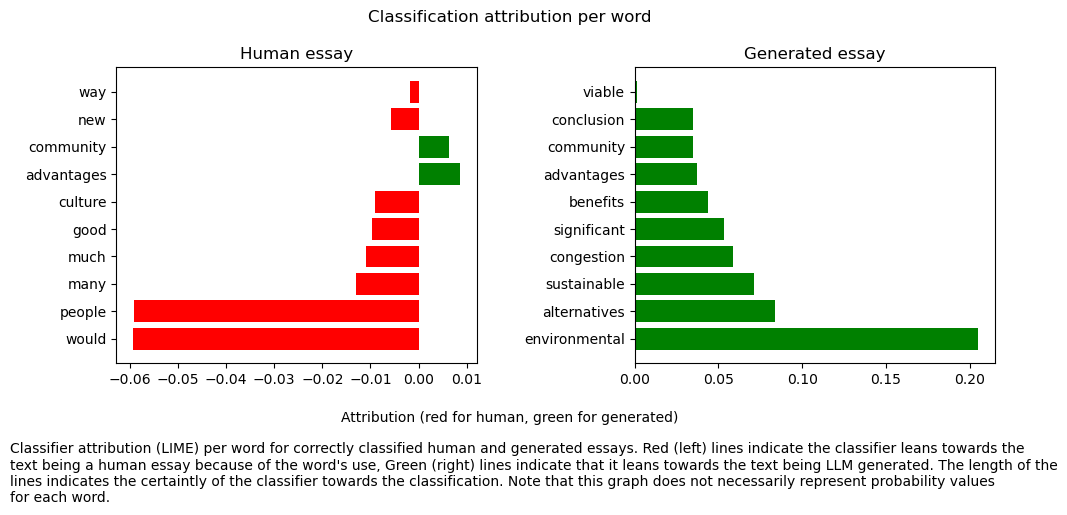
\includegraphics[width=14cm]{attribution.png}
		\centering
		\caption{Classifier attribution (LIME) per word for correctly classified human and generated essays. Red (left) lines indicate the classifier leans towards the text being a human essay because of the word's use, Green (right) lines indicate that it leans towards the text being LLM generated. The length of the lines indicates the certainty of the classifier towards the classification. Note that this graph does not necessarily represent probability values for each word.}
		\label{fig::attribution}
	\end{figure}
	
	\begin{figure}
		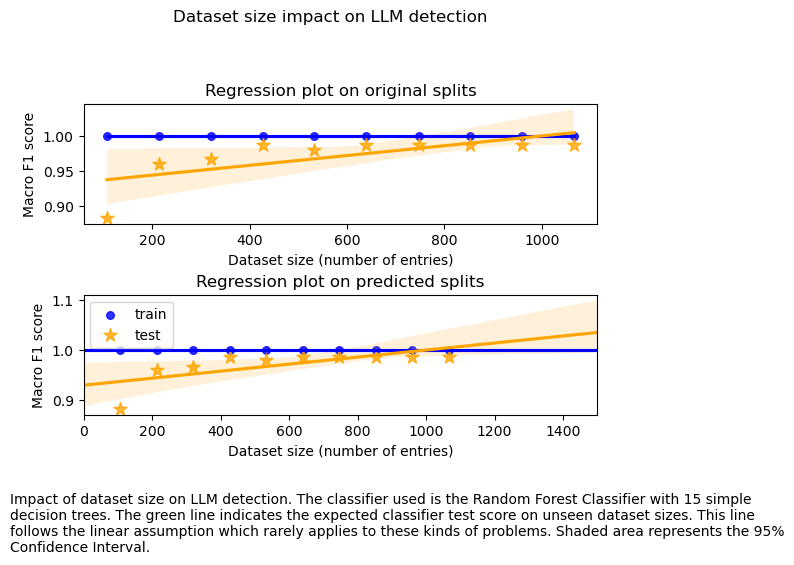
\includegraphics[width=14cm]{dataset_size.png}
		\centering
		\caption{Impact of dataset size on LLM detection. The classifier used is the Random Forest Classifier with 15 simple decision trees. The green line indicates the expected classifier test score on unseen dataset sizes. This line follows the linear assumption which rarely applies to these kinds of problems. Shaded area represents the 95\% Confidence Interval.}
		\label{fig::dataset_size}
	\end{figure}
	
	\begin{figure}
		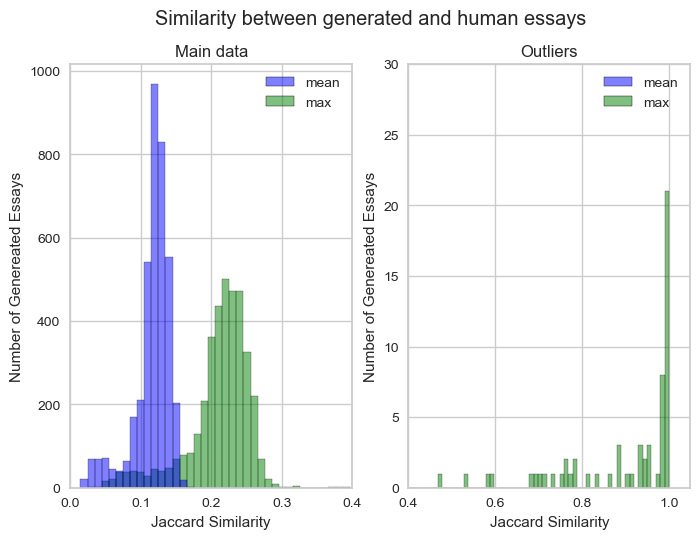
\includegraphics[width=14cm]{similarity.png}
		\centering
		\caption{Mean and maximum Jaccard similarity between each generated essay compared to all human essays. This Figure demonstrates the very low similarity between the two kinds of essays in our dataset, largely explaining the exceptional performance of our classifiers.}
		\label{fig::similarity}
	\end{figure}
	
	\begin{figure}
		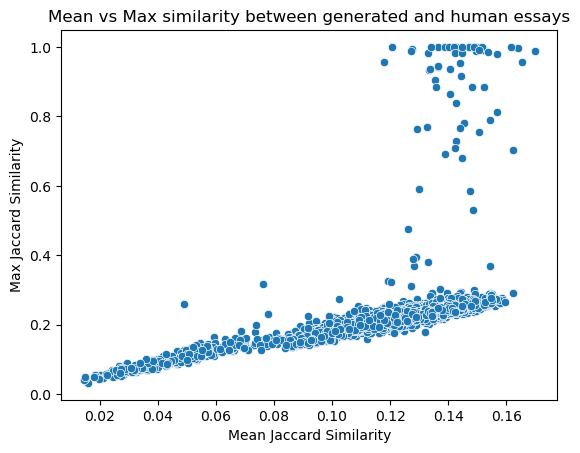
\includegraphics[width=14cm]{similarity_mean_max.png}
		\centering
		\caption{Relationship between mean and max similarity between each generated essay and all human essays. The relationship can be described as follows: From $0$ to $0.12$ mean similarity the relationship is clearly positive linear, while from $0.12$ to $0.20$ the relationship is still clearly positive and mostly linear but with significant outliers.}
		\label{fig::similarity_mean_max}
	\end{figure}
	
	\begin{figure}
		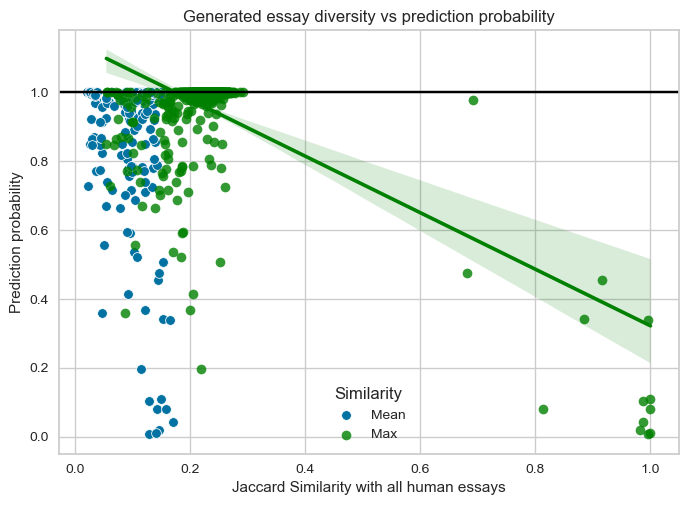
\includegraphics[width=14cm]{diversity_plot.png}
		\centering
		\caption{Relationship between essay similarity and prediction probability for that (generated) text. The distributions of mean and max similarity can also be seen in Figure \ref{fig::similarity}. We notice a slight inverse trend between max similarity and prediction probability. When similarity becomes 1, or very close to 1, the classifier fails since the data point itself is mislabeled.}
		\label{fig::diversity_plot}
	\end{figure}
	
	\begin{figure}
		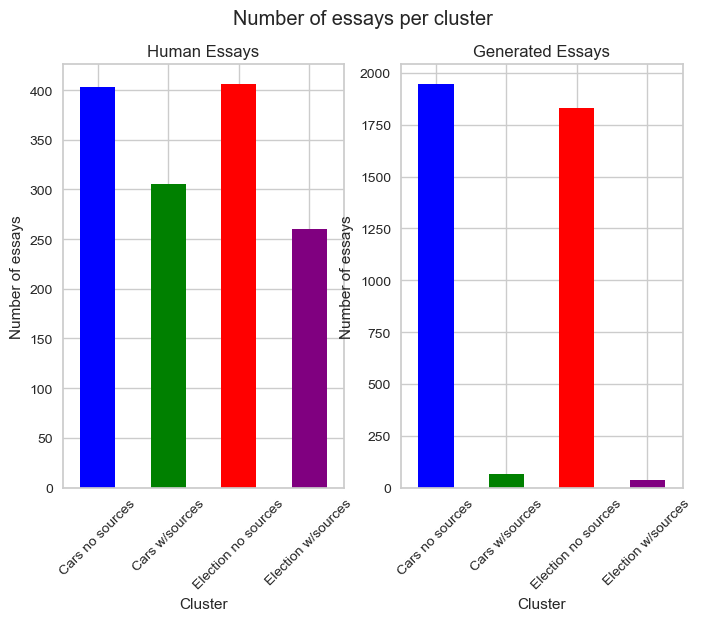
\includegraphics[width=14cm]{clusters.png}
		\centering
		\caption{K-Means clustering of human and generated essays, labeled according to qualitative characteristics. The optimal generated }
		\label{fig::clusters}
	\end{figure}
	
	\begin{figure}
		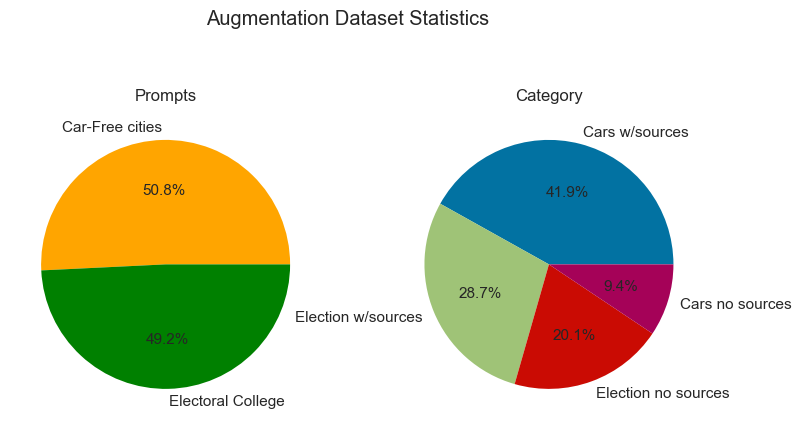
\includegraphics[width=14cm]{augmentation_stats.png}
		\centering
		\caption{Statistics about the final, full augmented dataset comprising all the generated essays, even those not eventually used for the final model. The "Category" pie-plot displays the relative counts of clusterings as defined by the K-means algorithm with $K=4$ trained on the human texts.}
		\label{fig::augmentation_stats}
	\end{figure}
\end{document}